\section{Numerical Results} \label{sec:res}
In this section we discuss the performance of the symplectic model-reduction with an energy inner product. In section \ref{sec:res.1} we apply the model reduction method to the equations of an elastic beam. We examine the evaluation of nonlinear terms in the model reduction of the nonlinear sine-Gordon equation, in section \ref{?}.

\subsection{The Elastic Beam Equation} \label{sec:res.1}
Consider the equations governing small deformations of a clamped elastic body $\Gamma\subset \mathbb R^{3}$ as 
\begin{equation} \label{eq:res.1}
\left\{
\begin{aligned}
	u_{tt}(t,x) &= \nabla \cdot \sigma + f, \quad & x\in \Gamma, \\
	u(0,x) &= \vec 0, & x\in \Gamma,\\
	\sigma \cdot n &= T, & x \in \partial \Gamma_T,\\
	u(t,x) &= \vec 0, & x \in\partial \Gamma \backslash \partial \Gamma_T,
\end{aligned}
\right.
\end{equation}
and
\begin{equation}  \label{eq:res.2}
	\sigma = \lambda (\nabla \cdot u) I + \mu(\nabla u + (\nabla u)^T).
\end{equation}
Here $u$ is the displacement vector field defined on $\Gamma$, subscript $t$ denotes derivative with respect to time, $\sigma$ is the stress tensor, $f$ is the body force per unit volume, $\lambda$ and $\mu$ are Lam\'e's elasticity parameters for material in $\Gamma$, $I$ is the identity tensor, $n$ is the outward unit normal vector at the boundary and $T:\partial \Gamma_T \to \mathbb R^3$ is the traction at the boundary $\partial \Gamma_T$ \cite{langtangen2017solving}.

We define a vector valued function space where we seek for the solution to (\ref{eq:res.1}) as $V = \{ u \in L^2(\Gamma) : \| \nabla u \|_2 \in L^2 \text{ and } u = \vec 0 \text{ on } \partial \Gamma_T \}$, equipped with the standard $L^2$ inner product $(\cdot,\cdot):V\times V \to \mathbb R$. To formulate the weak formulation of (\ref{eq:res.1}), we multiply it with the vector valued test function $v \in V$ and integrate over $\Gamma$
\begin{equation}  \label{eq:res.3}
	\int_{\Gamma} u_{tt} \cdot v\ dx = \int_{\Gamma} (\nabla \cdot \sigma) \cdot v \ dx + \int_{\Gamma} f \cdot v \ dx.
\end{equation}
We may integrate the first term on the right hand side by parts to obtain
\begin{equation}  \label{eq:res.4}
	\int_{\Gamma} u_{tt} \cdot v\ dx = - \int_{\Gamma} \sigma : \nabla v \ dx+ \int_{\partial \Gamma_T} (\sigma \cdot n) \cdot v\ ds +  \int_{\Gamma} f \cdot v \ dx,
\end{equation}
where $\sigma : \nabla v$ is the tensor inner product. Note that the skew-symmetric part of $\nabla v$ vanishes over the product $\sigma : \nabla v$, since $\sigma$ is symmetric. By prescribing the boundary conditions to (\ref{eq:res.4}) we recover
\begin{equation} \label{eq:res.5}
	\int_{\Gamma} u_{tt} \cdot v\ dx = - \int_{\Gamma} \sigma : \text{Sym}(\nabla v) \ dx+ \int_{\partial \Gamma_T} T \cdot v\ ds +  \int_{\Gamma} f \cdot v \ dx,
\end{equation}
with Sym$(\nabla v) = (\nabla v + (\nabla v)^T)/2$. The variational form associated to (\ref{eq:res.1}) then reads
\begin{equation} \label{eq:res.6}
	(u_{tt},v) = - a(u,v) + L(v), \quad u,v\in V,
\end{equation}
where
\begin{equation} \label{eq:res.7}
\begin{aligned}
	a(u,v) &= \int_{\Gamma} \sigma : \text{Sym}(\nabla v) \ dx, \\
	L(v) &= \int_{\partial \Gamma_T} T \cdot v\ ds +  \int_{\Gamma} f \cdot v \ dx.
\end{aligned}
\end{equation}
To obtain the finite element method (FEM) discretization of (\ref{eq:res.6}), we discretize the domain $\Gamma$ into a triangulated mesh, which discretizes the domain into a set of disjoint tetrahedrons. Furthermore, we define vector valued piece-wise linear basis functions $\{\phi_i\}_{i=1}^{N_h}$ and define the FEM space $V_h$ as an approximation of $V$ over these set of basis functions. Projecting (\ref{eq:res.6}) onto $V_h$ gives us the discretized weak form
\begin{equation} \label{eq:res.8}
	((u_h)_{tt},v_h) = - a(u_h,v_h) + L(v_h),\quad u_h,v_h\in V_h.
\end{equation}
Any particular function $u_h$ can be expressed as $u_h = \sum_{i=1}^{N_h} q_i \phi_i$, where $q_i$, $i=1,\dots,N_h$, are the expansion coefficients. Therefore, by choosing test functions $v_h = \phi_i$, $i=1,\dots,N_h$, we obtain the ordinary differential equation
\begin{equation} \label{eq:res.9}
	M\ddot q = -K q + g_{q}.
\end{equation}
where $q=(q_1,\dots,q_{N_h})^T$, $M\in \mathbb R^{N_h\times N_h}$ is given as $M_{i,j} = (\phi_i,\phi_j)$, $K\in \mathbb R^{N_h\times N_h}$ is given as $K_{i,j} = a(\phi_i,\phi_j)$ and $g_q=(L(v_1),\dots,L(v_{N_h}))^T$. We now introduce the canonical coordinate $p = M\dot q$ to recover the Hamiltonian system
\begin{equation} \label{eq:res.10}
	\dot z = \mathbb J_{2N_h} Lz + g_{qp}
\end{equation}
where
\begin{equation} \label{eq:res.11}
	z = 
	\begin{pmatrix}
	q \\
	p	
	\end{pmatrix}, \quad 
	L = 
	\begin{pmatrix}
	K & 0 \\
	0 & M^{-1}
	\end{pmatrix}, \quad
	g_{qp} =
	\begin{pmatrix}
	0 \\
	g_p
	\end{pmatrix},
\end{equation}
together with the Hamiltonian function $H(z) = z^TLz + z^T \mathbb J_{2N_h}^T g_{qp}$. A proper FEW set up leads to a symmetric and positive-definite matrix $L$. Therefore, it seams natural to take $X=L$, the energy matrix assciated to (\ref{eq:res.10}). System parameters are summarized in the table below. For further information regarding the problem set up, we refer the reader to \cite{langtangen2017solving}

\vspace{0.5cm}
\begin{center}
\begin{tabular}{|l|l|}
\hline
Domain shape & box: $l_x = 1,\ l_y = 0.2,\ l_z = 0.2$ \\
No. mesh points & $n_x = 10,\ n_y = 4,\ n_z = 4$ \\
Time discretization size & $\Delta t = 0.01$ \\
Gravitational force & $g = (0,0,-0.4)^T$ \\
Traction & $T = \vec 0$ \\
Lam\'e parameters & $\lambda = 1.25$, $\mu = 1.0$ \\
Degree of freedom & $2N_{h} = 1650$ \\
\hline
\end{tabular}
\end{center}
\vspace{0.5cm}

We used the St\"ormer-Verlet scheme (\ref{eq:hamil.6}) to integrate (\ref{eq:res.10}) in time and generate the time snapshots. Projection operators $P_{X,V}$, $P^{\text{symp}}_{I,A}$ and $P^{\text{symp}}_{X,A}$ are then constructed according to section {\ref{sec:mor.1}}, {\ref{sec:mor.2}} and {\ref{sec:mor.3}}, respectively. After computing the transformation $J_{2k} = T \mathbb J_{2k} T^T$, the reduced systems resulted from $P^{\text{symp}}_{I,A}$ and $P^{\text{symp}}_{X,A}$ are integrated in time using the St\"ormer-Verlet scheme. The reduced system yielded by $P_{X,V}$ is integrated using a second order implicit Runge-Kutta method. Note that the St\"ormer-Verlet scheme is not used since the canonical form of a Hamiltonian system will be is destroyed using $P_{X,V}$.

\begin{figure} \label{fig:1}
\begin{tabular}{cc}
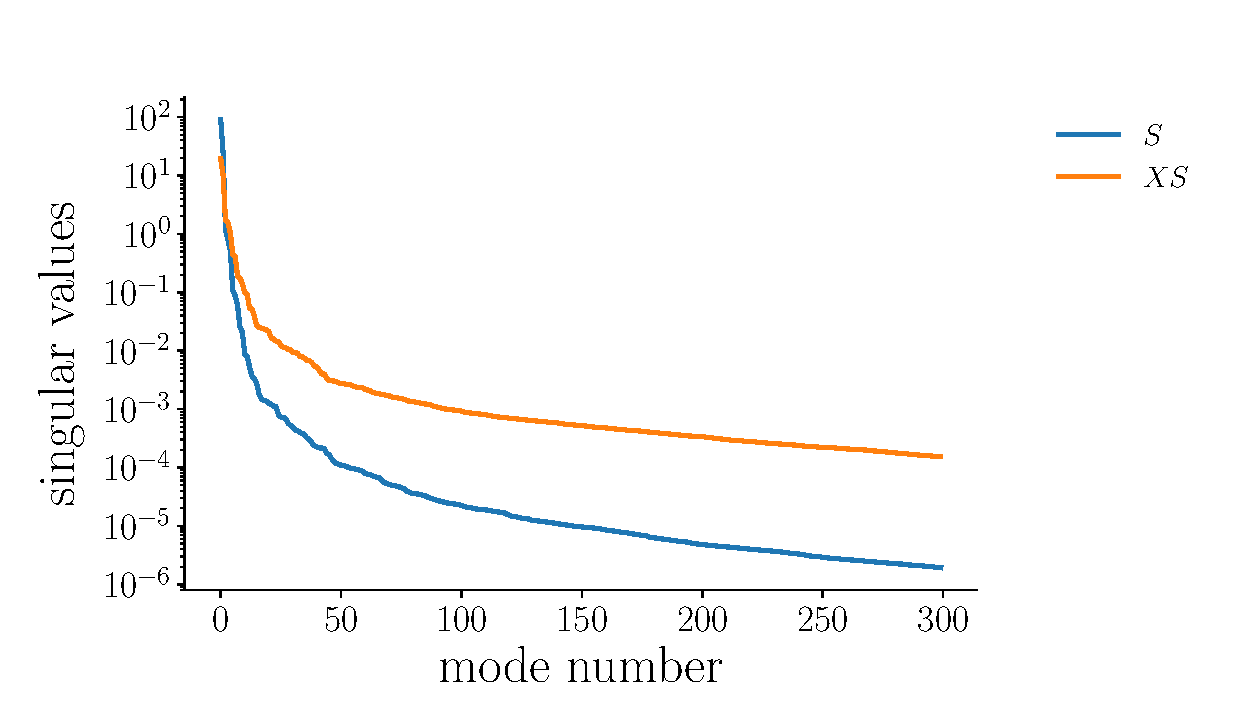
\includegraphics[width=0.45\textwidth]{./figs/beam/singulars} & 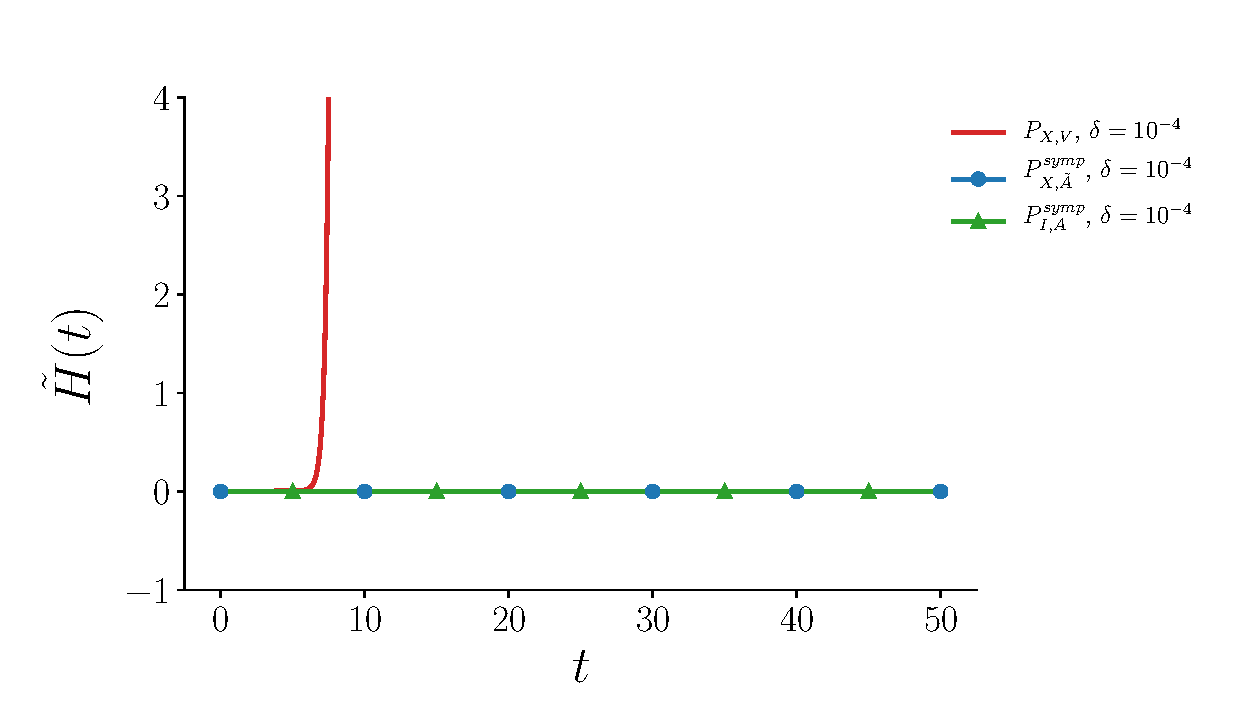
\includegraphics[width=0.45\textwidth]{./figs/beam/energy} \\
(a) & (b) \\
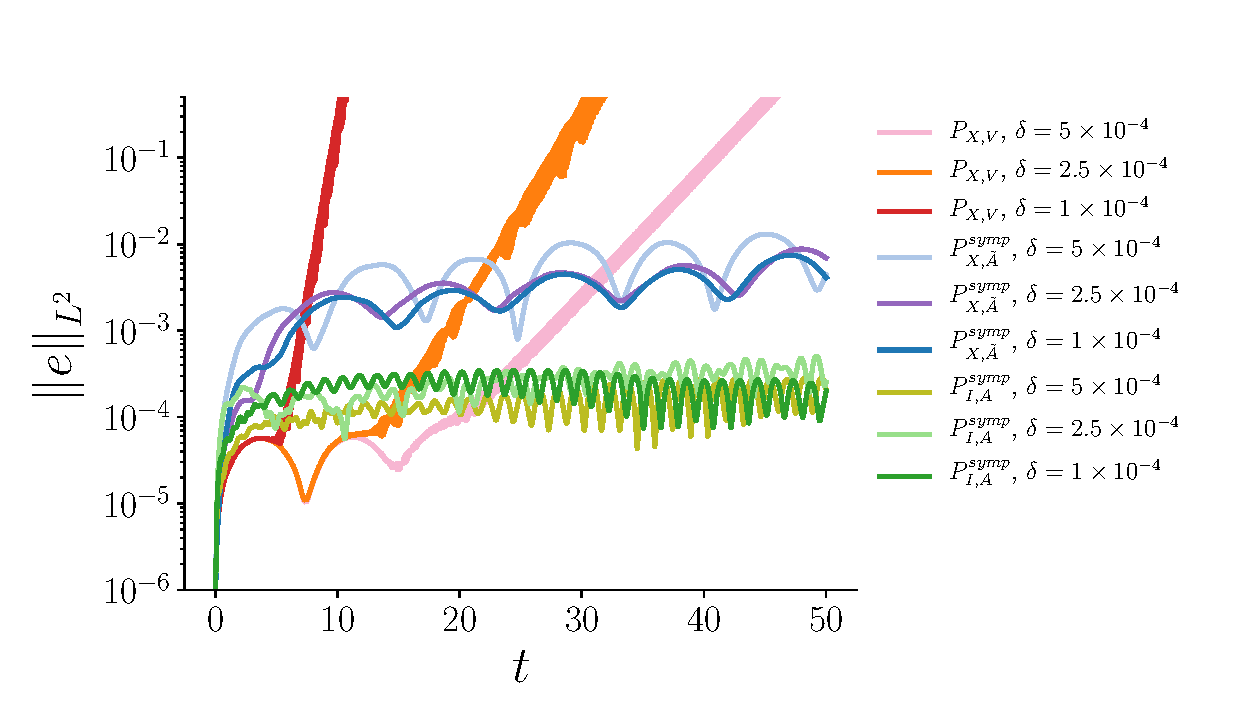
\includegraphics[width=0.45\textwidth]{./figs/beam/l2_norm} & 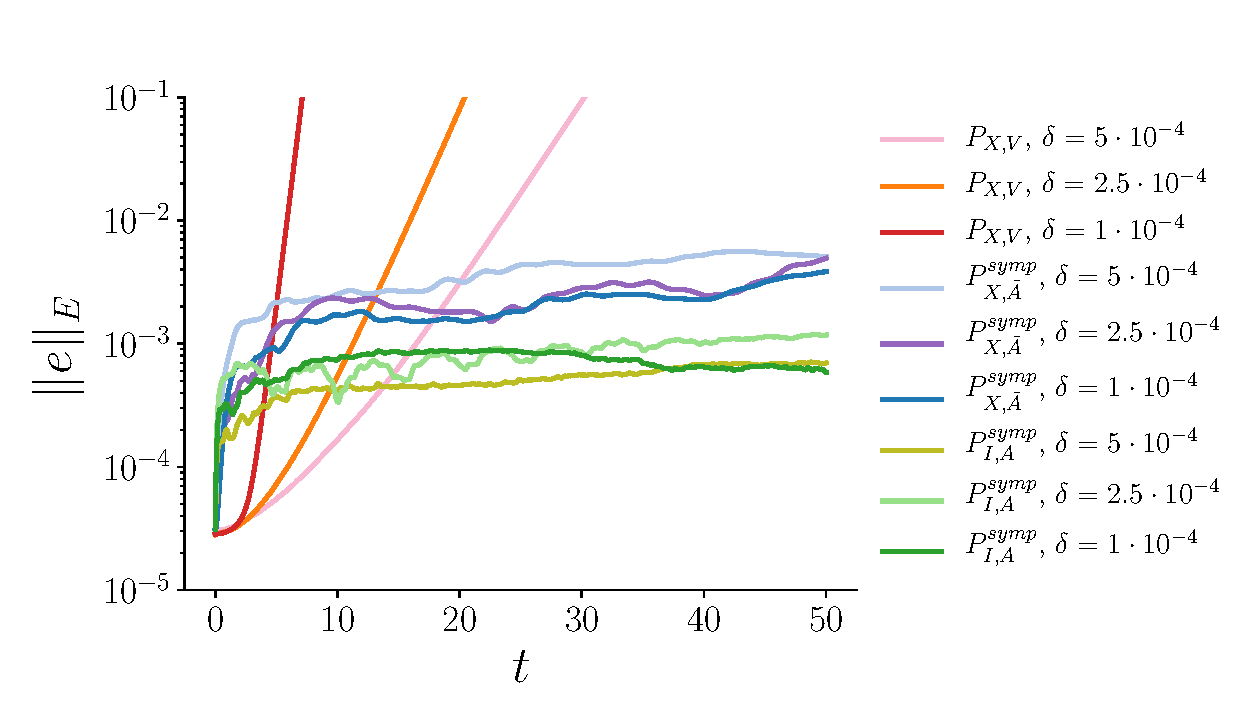
\includegraphics[width=0.45\textwidth]{./figs/beam/energy_norm} \\
(c) & (d) \\
\end{tabular}
\caption{(a) the decay of the singular values. (b) conservation of the Hamiltonian. (c) error with respect to the $L^2$ norm. (d) error with respect to the $X$-norm.}
\end{figure}

Figure \ref{fig:1}a show the decay of the singular values of the time snapshots $S$ and $X^{1/2}S$ respectively. We notice that the decay of the two matrices are different and as the matter of fact the decay saturates for $X^{1/2}S$.

Figure \ref{fig:1}b shows the conservation of the Hamiltonian for all methods mentioned above. It is observed that the symplectic methods do preserve the Hamiltonian and system energy. However, the Hamiltonian blows up for the reduced system constructed by the projection $P_{X,V}$. It is also noticeable that as the basis $V$ gets larger, the Hamiltonian blows up faster.

Figure \ref{fig:1}c shows the $L^2$ error of the reduced system generated by the projection. We notice that the reduced system obtained by the non-symplectic method is unstable. It is known that classical reduce basis methods generally become exceedingly unstable as the reduced basis is enriched. This can also be observed here as the reduced system constructed by $P_{X,V}$ is more unstable as $k$ increases. On the other hand, symplectic methods yield a stable reduced system. As the matter of fact, even as the system constructed by the projection $P^{\text{symp}}_{X,A}$ is not based on the $L^2$ projection, the error remains bounded with respect to the $L^2$ norm. 

Figure \ref{fig:1}d also indicates that classical model reduction methods based on the projection $P_{X,V}$ does not necessarily yield a stable reduced system. However, the symplectic methods provide a stable reduced system under long time-integration. We observe that the original symplectic also provide an accurate solution with respect to the $X$-norm. Nevertheless, the relation between the two norms are not generally known and in general depends on problem set up and initial and boundary conditions \cite{DEPARIS20094359}.

\subsection{The Sine-Gordon Equation} \label{sec:res.2}
The sine-Gordon equation arise in differential geometry and quantum physics \cite{Misumi2015}. This equation is a nonlinear generalization of the linear wave equation, given as
\begin{equation} \label{eq:res.12}
\left\{
\begin{aligned}
	u_{t}(t,x) &= v, \quad x\in \Gamma\\
	v_t(t,x) &= u_{xx} - \sin(u), \\
	u(t,0) &= 0 \\
	u(t,1) &= 1
\end{aligned}
\right.
\end{equation}
Here, $x\in \Gamma$ is an one dimensional box of length $L$, $u,v: \Gamma \to \mathbb R$ are scalar functions. The Hamiltonian associated to (\ref{eq:res.12}) is
\begin{equation} \label{eq:res.13}
	H(q,p) = \int_{\Gamma} \frac 1 2 v^2 + \frac 1 2 u_x^2 + 1 - \cos(u) \ dx.
\end{equation}
One can check that $u_{t} = \delta H / \delta v$ and $v_{t} = - \delta H / \delta u$. The sine-Gordon equation admits the solution solution
\begin{equation} \label{eq:res.14}
	u(t,x) = 4 \text{arctan}\left( \exp ( \pm \frac{x - x_0 - ct}{\sqrt{1-c^2}} ) \right),
\end{equation}
where the plus and minus signs are known as the \emph{kink} and \emph{anti-kink} solutions, respectively. Here $|c|<1$ is the wave speed. We discretize the box into $N$ equi-distant grid point $x_i = i\Delta x$, $i=1,\dots,N$. Furthermore, we use standard finite-differences schemes to discretize (\ref{eq:res.12}) to obtain
\begin{equation}
	\dot z = \mathbb J_{2n} L z + \mathbb J_{2n} g(z) + \mathbb J_{2n} c_b.
\end{equation}
Here $z = (q^T,p^T)^T$, $q(t) = (u(t,x_1),\dots,u(t,x_N))^T$, $p(t) = (v(t,x_1),\dots,v(t,x_N))^T$, $c_b$ is the term corresponding to the boundary conditions and
\begin{equation}
	L = 
	\begin{pmatrix}
		Dx^TDx & 0_N \\
		0_N & I_n
	\end{pmatrix}, 
	\quad
	g(z) = 
	\begin{pmatrix}
	\sin(q) \\
	\vec 0
	\end{pmatrix},
\end{equation}
where $Dx$ is the standard matrix differentiation operator. The discrete Hamiltonian, then takes the form
\begin{equation}
	H_{\Delta x} = \Delta x \cdot \frac 1 2 \| p \|^2 + \Delta x \cdot \| D_x q \|^2 + \sum_{i=1}^{N} \Delta x \cdot ( 1 - \cos(q_i) ).
\end{equation}
The system parameters can be found in the table below.
\vspace{0.5cm}
\begin{center}
\begin{tabular}{|l|l|}
\hline
Domain legnth & box: $L = 50$ \\
No. grid points & $n = 250$ \\
Time discretization size & $\Delta t = 0.01$ \\
Wave speed & $c=0.2$ \\
\hline
\end{tabular}
\end{center}
\vspace{0.5cm}

The St\"ormer-Verlet Scheme is used to integrate (\ref{eq:res.12}) in time and generate the snapshot matrix $S$. Similar to the previous subsection, projection operators $P_{X,V}$, $P^{\text{symp}}_{I,A}$ and $P^{\text{symp}}_{X,A}$ are used to construct a reduced system. To accelerate the evaluation of the nonlinear term, the symplectic methods discussed in section (\ref{eq:mor.1}) and (\ref{eq:mor.2}) are coupled with the projection operators $P^{\text{symp}}_{I,A}$ and $P^{\text{symp}}_{X,A}$, respectively. Furthermore, the DEIM approximation is used for efficient evaluation of the reduced system obtained by the projection $P_{X,V}$. The time-stepping scheme used to integrate the reduced systems are taken identical to the ones in section (\ref{sec:res.1})
